%%%%%%%%%%%%%%%%%%%%%%%%%%%%%%%%%%%%%%%%%%%%%%%%%%%%%%%%%%%%%%%%%%%%%%%%%%%%%%%%
% Лабораторная работа 2 : Измерение модуля Юнга и коэффициента Пуассона.
% Выполнили             : Баталов Семен, Хайретдинова Диана, 2021.
%%%%%%%%%%%%%%%%%%%%%%%%%%%%%%%%%%%%%%%%%%%%%%%%%%%%%%%%%%%%%%%%%%%%%%%%%%%%%%%%

\documentclass[12pt, a4paper]{article}
\usepackage[left=2cm, right=2cm, top=2.5cm, bottom=2.5cm, nohead]{geometry}
\usepackage{graphicx}
\usepackage[utf8]{inputenc}
\usepackage[english, russian]{babel}
\usepackage{indentfirst}
\usepackage{amsmath}
\usepackage{longtable}
\usepackage{multirow}
\usepackage{array}
\usepackage{rotating}
\usepackage{subcaption}
\graphicspath{{./Figures/}}

\begin{document}
    
    \newcolumntype{M}[1]{>{\centering\arraybackslash}m{#1}}
    \renewcommand{\arraystretch}{1.4}
    
    \begin{center}
        \large{Санкт-Петербургский Государственный Университет} \\
        \large{Saint-Petersburg State University}\\
        \hfill \break
        \hfill \break
        \hfill \break
        \hfill \break
        \hfill \break
        \hfill \break
        \large{ЛАБОРАТОРИЯ ПРОЧНОСТИ МАТЕРИАЛОВ} \\
        \hfill \break
        \hfill \break
        \hfill \break
        \large{\textbf{ОТЧЕТ}} \\
        \large{\textbf{По лабораторной работе 2}} \\
        \large{<<Измерение модуля Юнга и коэффициента Пуассона>>} \\
        \hfill \break
        \hfill \break
        \hfill \break
        \large{По дисциплине} \\
        \large{<<Лабораторный практикум, лабораторная работа>>} \\
    \end{center}
    
    \hfill \break
    \hfill \break
    \hfill \break
    \hfill \break
    \hfill \break
    \hfill \break
    
    \begin{flushright} 
        \large{Выполнили:} \\
        \hfill \break
        \large{Баталов С. А.} \\
        \large{Хайретдинова Д. Д.} \\
    \end{flushright}
    
    \hfill \break
    \hfill \break
    \hfill \break
    \hfill \break
    \hfill \break
    \hfill \break
    
    \begin{center} 
        \large{Санкт-Петербург} \\
        \large{2021} \\
    \end{center}
    
    \thispagestyle{empty}
    \newpage
    \sloppy
    
    \section{Цель работы}
    
    Механизм упругого деформирования материалов состоит в обратимых смещениях атомов из положений равновесия в кристаллической решетке. Чем больше величина смещения каждого атома, тем больше упругая деформация тела. Величина упругой деформации невелика и для металлов и для их сплавов меньше 1\%.
    
    Поведение материалов при упругой деформации описывается законом Гука, который определяет прямую пропорциональную зависимость между компонентами тензоров деформации и напряжения.
    
    В данной лабораторной работе производится исследование образцов на растяжение с измерением деформаций и определением постоянных, характеризующих упругие свойства образца~--~модуля Юнга $E$ и коэффициента Пуассона $\nu$. При измерении деформаций используют проволочные тензодатчики сопротивления (ТД).
    
    \newpage
    
    \section{Теоретические исследования}
    
    Рассмотрим стержень длины $l = 150~\text{мм}$, ширины $a = 28.7~\text{мм}$ и толщины $b = 2.2~\text{мм}$. Площадь сечения пластины равна $S_{0} = 63~\text{мм}^{2}$, стержень растягивается силой $P$.
    
    \begin{figure}[h]
        \centering
        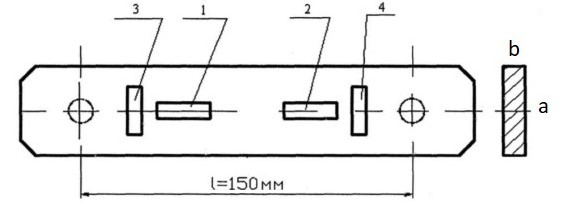
\includegraphics[width = 12cm]{image_1.jpg}
        \caption{Испытательная пластина.}
        \label{im1}
    \end{figure}
    
    Пусть ось $Ox$ системы координат совпадает с осью стержня. Стержень будет находиться в состоянии одноосного растяжения, то есть напряжения в 
    нем будут равны:
    
    \begin{equation}
        \sigma_{xx} = \frac{P}{S_{0}}; \quad \sigma_{yy} = \sigma_{zz}			=\sigma_{xy} = \sigma_{xz} = \sigma_{yz} = 0.
        \label{eq1}
    \end{equation}
    
    Знаем, что поведение материалов при упргой деформации описывается законом Гука, в общем случае закон Гука записывается следующим образом:
    
    \begin{equation}
        \begin{aligned}
            \varepsilon_{xx} = \frac{1}{E}\Big(\sigma_{xx} - \nu(\sigma_{yy} + \sigma_{zz})\Big); \quad \sigma_{xy} = \frac{E}{1 + \nu}\varepsilon_{xy};
            \\
            \varepsilon_{yy} = \frac{1}{E}\Big(\sigma_{yy} - \nu(\sigma_{xx} + \sigma_{zz})\Big);\quad  \sigma_{yz} = \frac{E}{1 + \nu}\varepsilon_{yz};
            \\
            \varepsilon_{zz} = \frac{1}{E}\Big(\sigma_{zz} - \nu(\sigma_{yy} + \sigma_{xx})\Big); \quad \sigma_{xz} = \frac{E}{1 + \nu}\varepsilon_{xz}.
        \end{aligned}
        \label{eq2}
    \end{equation}
    
    Подставив (\ref{eq1}) в (\ref{eq2}), получим, что при данном поле напряжений относительные удлинения по всем осям будут отличны от нуля, а сдвиги будут равны нулю:
    
    \begin{equation}
        \varepsilon_{xx} = \frac{1}{E}\sigma_{xx}; \quad \varepsilon_{yy} = \varepsilon_{zz}= - \frac{\nu}{E}\sigma_{xx}; \quad \varepsilon_{xy} = \varepsilon_{yz} = \varepsilon_{xz} = 0.
        \label{eq3}
    \end{equation}
    
    Отсюда получим, что экспериментальным путем модуль Юнга и коэффициент Пуассона может быть получен по следующим формулам:
    
    \begin{equation}
        E = \frac{P}{S_{0}}\frac{1}{\varepsilon_{xx}}; \quad \nu = - \frac{\varepsilon_{yy}}{\varepsilon_{xx}}.
        \label{eq4}
    \end{equation}
    
    Относительные удлинения $\varepsilon_{xx}$ и $\varepsilon_{yy}$ стержня в данной работе находим прямым измерением при помощи тензодатчиков.
    
    \newpage
    
    \section{Экспериментальная установка}
    
    В данной лабораторной работе деформации измеряются посредством тензодатчиков, которые установлены в продольном и поперечном направлениях. Тензодатчик (рис.~\ref{im2}) состоит из зигзагообразно уложенной проволоки (решетки) \textit{1}, наклеенной на подложку (тонкую бумагу) \textit{2}. К концам проволочной решетки припаяны медные выводы \textit{3}. Сверху решетка покрыта защитным слоем бумаги или лака. Тензодатчик измеряет относительное удлинение в направлении, обозначенном стрелками (рис.~\ref{im2}).
    
    \begin{figure}[h]
        \centering
        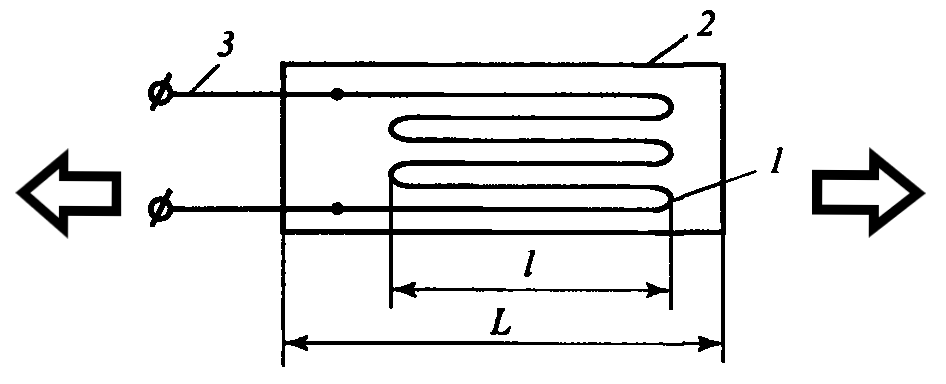
\includegraphics[width = 12cm]{image_2.png}
        \caption{Схема тензодатчика.}
        \label{im2}
    \end{figure}
    
    На рисунке (\ref{im1}) тензодатчики \textit{1} и \textit{2} измеряют продольное удлинение, \textit{3} и \textit{4} поперечное. Тензодатчики подключены к электронному измерителю деформации. Чувствительность датчика характеризуется коэффициентом $K = 6.4 \cdot 10^{-7}$.
    
    Лабораторная работа выполняется на универсальном лабораторном 
    стенде по сопротивлению материалов (рис.~\ref{im3}), здесь \textit{1}~--~образец, \textit{2}~--~нагружающее устройство, \textit{3}~--~силоизмерительное устройство.
    
    \begin{figure}[h]
        \centering
        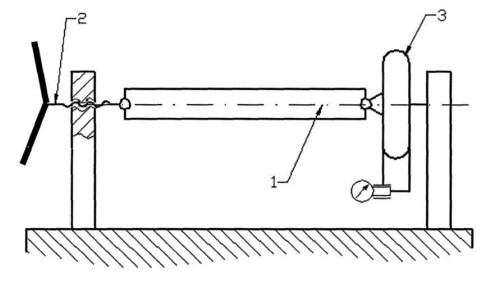
\includegraphics[width = 12cm]{image_3.jpg}
        \caption{Схема экспериментальной установки.}
        \label{im3}
    \end{figure}
    
    \newpage
    
    \section{Эксперимент}
    
    При выполнении работы расчеты производились с помощью инструментов пакета Matlab. Образец нагружали последовательно силой $P$ до $500~\text{Н}$ с шагом $50~\text{Н}$, на каждом шаге фиксировались показания измерителя деформаций для всех тензорезистров. Подсчитали разность показаний прибора для ступени $\Delta P = 50~\text{Н}$ и занесли в таблицу~\ref{tb1}. Все показания были усреднены. Для каждого шага были вычислены постоянные $\nu$ и $E$. Относительные деформации $\varepsilon_{xx}$, $\varepsilon_{yy}$, соответствующие приращениям силы, были определены по следующим формулам:
    
    \begin{equation}
        \varepsilon_{xx} = \Delta n_{x} \cdot K; \quad \varepsilon_{yy} = \Delta n_{y} \cdot K.
    \end{equation}
    
    Далее построим график зависимости напряжения $\sigma_{xx}$ от величины продольной деформации $\varepsilon_{xx}$. Построим прямую методом наименьших квадратов.
    
    \begin{figure}[h]
        \centering
        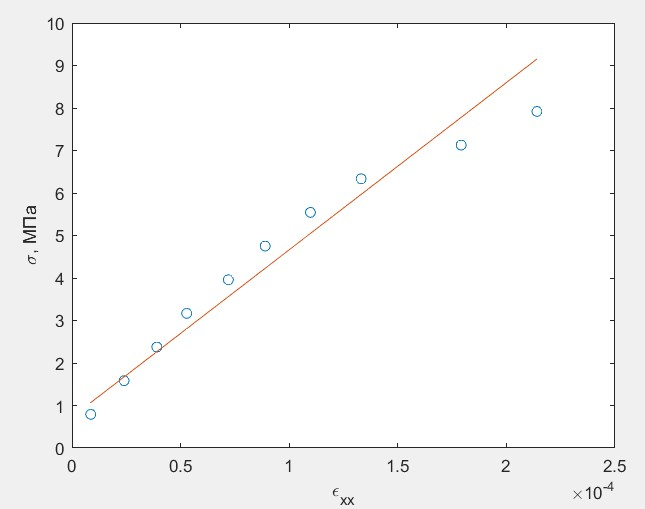
\includegraphics[width = 10cm]{image_4.jpg}
        \caption{График зависимости $\sigma_{xx}$ от $\varepsilon_{xx}$.}
        \label{im4}
    \end{figure}
    
    Считая, что в двух последних шагах результаты не являются достоверными, были вычислены конечные значения коэффициента Пуассона $\nu$ и модуля Юнга $E$. Все погрешности и окончательные результаты измерений модуля Юнга и коэффициента Пуассона представлены в следующей таблице:
    
    \begin{table}[h]
        \centering
        \begin{tabular}{| M{3cm} | M{3cm} | M{3cm} |}
            \hline
            Величина & Значение & Размерность \\
            \hline
            $E$ & 51 & \multirow{2}{*}{ГПа} \\
            $\Delta E$ & 12 & \\
            \hline
            $\nu$ & 0.32 & \multirow{2}{*}{--} \\
            $\Delta \nu$ & 0.01 & \\
            \hline
            $\Delta E / E$ & 23 & \multirow{2}{*}{\%} \\
            $\Delta \nu / \nu$ & 2 & \\
            \hline
        \end{tabular}
    \end{table}
    
    \newpage
    
    \section{Выводы}
    
    В проделанной работе мы исследовали на практике одноосное растяжение стержня, измеряя деформации при помощи тензодачиков, подключенных к измерителю деформаций. Познакомились с принципом работы тезодатчиков сопротивления, их преимуществами и недостатками. Исследовав изменение продольной деформации при увеличении нагрузки, убедились в линейной зависимости продольной деформации от напряжения. Вычислили модуль Юнга и коэффициент Пуассона. Оценили относительные и абсолютные погешности результатов.
    
    \newpage
    
    \begin{table}[h]
        \centering
        \begin{tabular}{|M{1.5cm}|M{1.5cm}|M{1.5cm}|M{1.5cm}|M{1.5cm}|M{1.5cm}|M{1.5cm}|M{1.5cm}|}
            \hline
            $P$ & $\Delta n_{x}$ & $\Delta n_{y}$ & $\varepsilon_{xx}$ &
            $\varepsilon_{yy}$ & $\sigma_{xx}$ & $\nu $& $E$ \\
            \hline
            Н & \multicolumn{2}{c|}{дел.} & \multicolumn{2}{c|}{$10^{-6}$} & МПа & -- & ГПа \\
\hline
	50&14&-6&8.64&-3.52&0.79&0.43&88.38\\

	100&24&-7&15.36&-4.16&1.58&0.29&51.56\\

	150&24&-9&15.04&-5.76&2.38&0.37&51.56\\

	200&22&-5&13.76&-2.88&3.17&0.23&56.24\\

	250&30&-11&19.2&-6.72&3.96&0.37&41.24\\

	300 & 27 & -8 & 16.96 & -4.8 & 4.75 & 0.3 & 45.83\\

	350&33&-9&20.8&-5.76&5.54&0.27&37.49\\

	400&37&-10&23.36&-6.08&6.34&0.27&33.44\\

	450&72&-23&46.08&-14.4&7.13&0.32&17.19\\

	500 & 55 & -16 & 34.88 &-9.92 &7.92 & 0.29 & 22.5\\
\hline
        \end{tabular}
        \caption{Экспериментальные и расчетные данные.}
        \label{tb1}
    \end{table}
    
\end{document}